\section{Вычисление факториала}

\textbf{Задание:} Разработать приложение для вычисления факториала по приведенному примеру.

Создано окно приложения, содержащее два элемента TextBox, два элемента Label и один элемент Button. Для отображения сообщений об ошибках
в окно добавлен элемент ErrorProvider. Вид окна представлен на рисунке \ref{fig:task1_form}.
\begin{figure}[H]
    \centering
    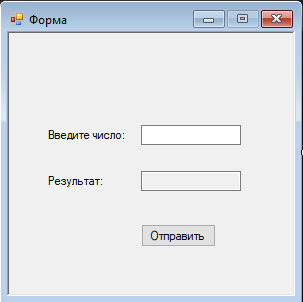
\includegraphics{task1/form.png}
    \caption{Внешний вид формы программы для вычисления факториала}
    \label{fig:task1_form}
\end{figure}
У элементов изменены значения некоторых атрибутов. 
Значения измененных атрибутов представлены в таблице \ref{table:params1}.

\begin{table}[H]
    \small
    \caption{Значения атрибутов элементов в приложении <<Факториал>>}\label{tab:fact-attr}
    \begin{tabular}{|l|l|}\hline
    Наименование атрибута & Значение\cr\hline
    \multicolumn{2}{|l|}{Для формы}\cr\hline
    \verb"Text" & \verb"Форма"\cr\hline
    \verb"FormBorderStyle" & \verb"FixedSingle"\cr\hline
    \verb"MaximizeBox" & \verb"False"\cr\hline
    \multicolumn{2}{|l|}{Для первой надписи}\cr\hline
    \verb"(Name)" & \verb"lblInput"\cr\hline
    \verb"Text" & \verb"Введите целое число"\cr\hline
    \multicolumn{2}{|l|}{Для второй надписи}\cr\hline
    \verb"(Name)" & \verb"lblOutput"\cr\hline
    \verb"Text" & \verb"Результат"\cr\hline
    \multicolumn{2}{|l|}{Для первого текстового поля}\cr\hline
    \verb"(Name)" & \verb"txtInput"\cr\hline
    \multicolumn{2}{|l|}{Для второго текстового поля}\cr\hline
    \verb"(Name)" & \verb"txtOutput"\cr\hline
    \multicolumn{2}{|l|}{Для кнопки}\cr\hline
    \verb"(Name)" & \verb"btnCalculate"\cr\hline
    \verb"Text" & \verb"Вычислить"\cr\hline
    \multicolumn{2}{|l|}{Для обработчика ошибок}\cr\hline
    \verb"(Name)" & \verb"errorProvider1"\cr\hline
    \end{tabular}
    \label{table:params1}
\end{table}

Для работы программы была написана функция вычисления факториала:
\inputminted[fontsize=\small, breaklines=true, style=bw, linenos]{cpp}{task1/fact.h}
Здесь переменная \verb|N| "--- число, для которого нужно вычислить факториал.

На нажатие кнопки <<Вычислить>> установлено выполнение следующего
кода:
\begin{minted}[fontsize=\small, breaklines=true, style=bw, linenos]{cpp}
    private: System::Void btnCalculate_Click(System::Object^ sender, System::EventArgs^ e) {
		ClearAll();
		ll InputNumber;
		bool result = Int64::TryParse(txtInput->Text, InputNumber);
		if (!result) {
			errorProvider1->SetError(txtInput, "Введено не целое число");
			return;
		}
		if (InputNumber > 20) {
			errorProvider1->SetError(txtInput, "Число слишком большое");
			return;
		}
		ll OutputNumber = fact(InputNumber);
		if (OutputNumber == -1) {
			errorProvider1->SetError(txtInput, "Введено отрицательное число");
			return;
		}
		txtOutput->Text = System::Convert::ToString(OutputNumber);
	}
\end{minted}

После запуска приложения на экране появляется окно (см. рисунок \ref{fig:exec1})
\begin{figure}[H]
    \centering
    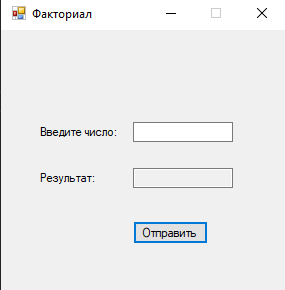
\includegraphics{task1/exec.png}
    \caption{Скриншот запуска программы}
    \label{fig:exec1}
\end{figure}

При вводе целого числа после нажатия кнопки в поле вывода приводится
результат вычисления факториала для заданного числа (см. рисунок \ref{fig:result1}).
\begin{figure}[H]
    \centering
    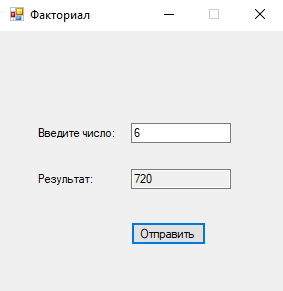
\includegraphics{task1/result.png}
    \caption{Результат работы}
    \label{fig:result1}
\end{figure}

Ввод некорректных значений обрабатывается элементом \verb|errorProvider1| и 
сопровождается сообщением об ошибке (см. рисунок \ref{fig:error1} )
\begin{figure}[H]
    \centering
    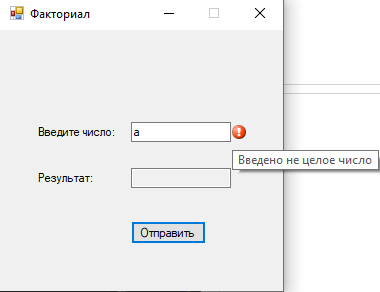
\includegraphics{task1/error.png}
    \caption{Сообщение об ошибке}
    \label{fig:error1}
\end{figure}
Полный код программы приведен в приложении А.